\chapter{Goal Oriented Action Planning}
\label{chap:goap}

Das folgende Kapitel wird die Funktionsweise von GOAP beschreiben. Es geh\"{o}rt zu den dynamischen Entscheidungssystemen in der Game-AI. Die Aktionen sind dabei nicht statisch verbunden, wie in den Ad-Hoc Behavioring Authoring Methoden. Es ist f\"{u}r die Planung an Aktionen zu einem bestimmten Ziel gedacht. Planung ist der Prozess der Suche einer Sequenz an Aktionen zur Erreichung eines Zieles. Die Suche kann dabei als Suchproblem dargestellt werden und durch Suchalgorithmen gel\"{o}st werden. F\"{u}r das Verst\"{a}ndnis werden Kenntnisse der Themen Suchalgorithmen und Suchprobleme des Kapitel \ref{chap:suchproblem und suchalgorithmen} erfordert.

\section{Historie}
\label{chap:goap historie}

Das Entscheidungssystem GOAP entstand in der Entwicklung des Videospiel F.E.A.R durch das Entwicklerstudio Monolith. Die Entwickler wollten ein Videospiel entwickeln, das wie ein Actionfilm wirkt, mit intensiven K\"{a}mpfen. F\"{u}r die intensiven K\"{a}mpfe ben\"{o}tigt man NPC, welche Deckung nehmen, blind feuern, \"{u}ber Fenster springen, Granaten werfen, untereinander kommunizieren und weitere Aktionen ausf\"{u}hren k\"{o}nnen.\autocite{fear}

Zuvor nutzte Monolith FSMs als Entscheidungssystem. Den Entwicklern fiel es jedoch zunehmend aufwendig, eine FSM mit neuen Zust\"{a}nden und den dazugeh\"{o}rigen Aktionen zu erweitern. In einem vorherigen Videospiel No One Lives Forever (2000), wurde veruscht eine dynamische FSM zu implementieren, die sich an Zielzust\"{a}nde anpassen konnte. Allerdings wurde auch diese L\"{o}sung als zu unflexibel wahrgenommen. Aus dem Versuch der dynamischen FSM und STRIPS hat Jeff Orkin das GOAP System entwickelt, welches Echtzeitplanung erf\"{u}llen soll. Eine der Herausforderungen, mit denen sich Jeff Orkin w\"{a}hrend der Entwicklung konfrontiert sah, war die Ber\"{u}cksichtigung der Performance.\autocite{retro_fear}



\section{GOAP Bestandteile}
\label{chap:goap bestandteile}

Das GOAP -System basiert dabei auf dem STRIPS System und wurde von Jeff Orkin entwickelt. Wie auch STRIPS besitzt GOAP Ziele, welche einen gew\"{u}nschten Zustand beschreiben und Goap-Aktion mit Effekten die Zust\"{a}nde \"{a}ndern k\"{o}nnen. GOAP sucht nach einer Sequenz an Goap-Aktion, der Aktions-Sequenz, die das Ziel des NPC erreichen kann. Im Sinne von Jeff Orkins geschieht die eigentliche Ausf\"{u}hrung der Aktionen \"{u}ber eine FSM. Die Informationen zu den Grundlagen kommen aus \autocite{fear, fear2, fear3}


\subsection{Finite State Machine in GOAP}
\label{chap:fsm goap}

Das Videospiel F.E.A.R (2005) ben\"{o}tigt f\"{u}r die Ausf\"{u}hrung der Aktionen eine FSM. Die NPCs f\"{u}hren ihre Aktionen durch eine Kombination aus Animationen und Bewegungen aus. Beispielsweise sorgt eine Cover-Aktion daf\"{u}r, dass der NPC hinter eine Deckung l\"{a}uft und dort eine Deckungs-Animation abspielt. Eine Shoot-Aktion hingegen aktiviert eine entsprechende Schuss-Animation. Die FSM besteht dabei aus den drei Zust\"{a}nden GoTo, Animate und UseSmartObject. 
\begin{figure}[h]
  \centering
  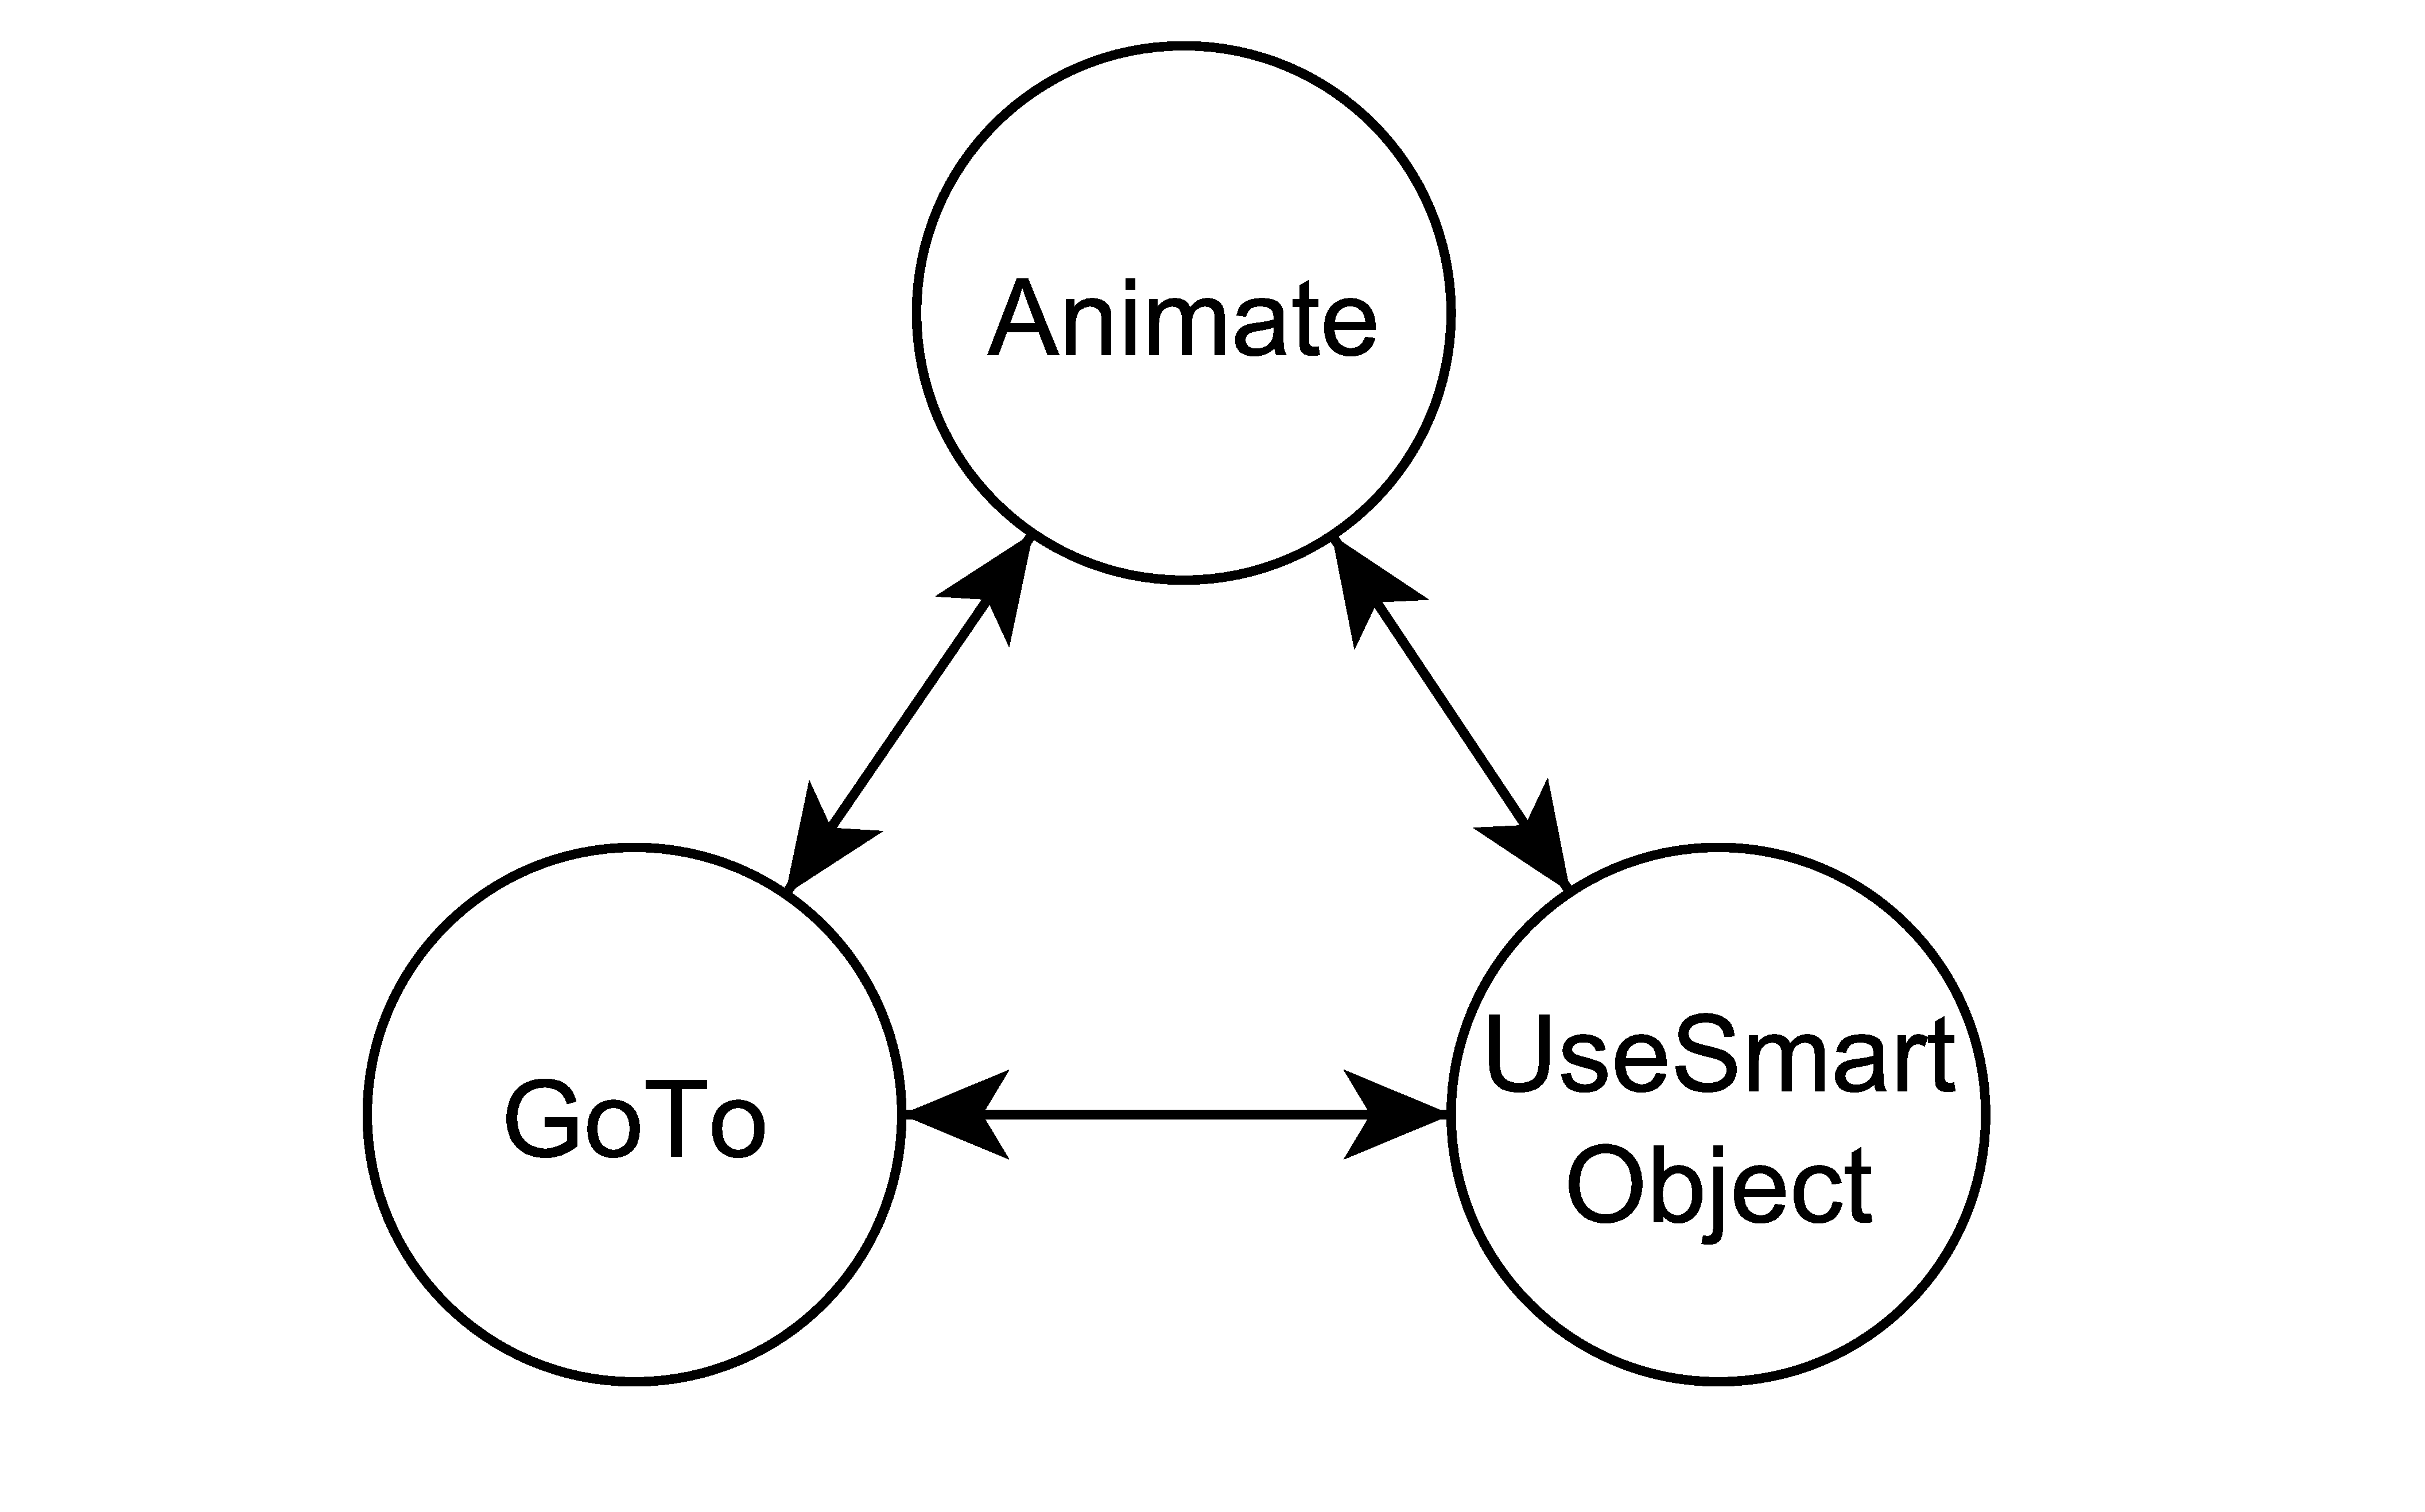
\includegraphics[width=0.7\textwidth]{GOAP/fsm.pdf}
	\captionsetup{justification=justified, format=plain}
  \caption{GOAP Finite State Machine}
  \label{fig:Goap FSM}
\end{figure}

Die Monolith-Entwickler hat durch die Zust\"{a}nde \textit{Animate} und \textit{UseSmartObject} Animationen umgesetzt. Der Unterschied zwischen den beiden Zust\"{a}nden besteht darin, dass \textit{UseSmartObject} Animationen steuert, die von \textit{SmartObjects} in der Spielwelt vorgegeben werden, w\"{a}hrend \textit{Animate} Animationen abspielt, die direkt im NPC gespeichert sind. Der Zustand \textit{GoTo} hat ebenfalls Animationen abgespielt, kombiniert diese jedoch mit der tats\"{a}chlichen Bewegung des NPCs durch die Spielwelt.

Die Zustandswechsel werden durch die Goap-Aktion bestimmt, welche wiederum durch GOAP gegeben werden.


\subsection{GOAP Ziele}
\label{chap:goap ziele}

Ein Ziel \textit{GOAL}$(g)$ in GOAP setzt die erw\"{u}nschte Zielzust\"{a}nde f\"{u}r den Planer. So setzt das Ziel \textit{EliminatePlayer} den Zielzustand $\{\lnot \textit{PlayerAlive}\}$.

\begin{align}
	\textit{GOAL}(\textit{EliminatePlayer}) = \{\lnot \textit{PlayerAlive}\}
\end{align}


Die Auswahl des Zieles geschieht nach ihrer Priorit\"{a}t und ob dieses g\"{u}ltig ist. Das Ziel mit der h\"{o}chsten Priorit\"{a}t und G\"{u}ltigkeit wird bevorzugt. Die G\"{u}ltigkeit und Priorit\"{a}t basiert dabei auf dem Zustand $s$ des NPC und seiner Umwelt. So ist das Ziel \textit{EliminatePlayer} mit dem Zustand $s$ nicht g\"{u}ltig und besitzt eine hohe Priorit\"{a}t.

\begin{align}
	s = \{\lnot \textit{PlayerVisible}\} \\
	\textit{PRIORITY}(s,\textit{EliminatePlayer}) = 100 \\
	\textit{VALID}(s,\textit{EliminatePlayer}) = \textit{false}
\end{align}


\subsection{GOAP Aktionen}
\label{chap:goap actions}

Die Goap-Aktion k\"{o}nnen Weltzust\"{a}nde oder auch direkte Zust\"{a}nde eines NPC \"{a}ndern. So kann beispielsweise die Goap-Aktion \textit{Reload} den Zustand $s = \{\lnot \textit{GunLoaded}\}$ mit seinem Effekt \"{a}ndern.

\begin{align}
	\textit{TRANSITIONS}(s,\textit{Reload}) &= \{\textit{GunLoaded}\}
\end{align}


Dadurch haben Goap-Aktion die M\"{o}glichkeit Zielzust\"{a}nde zu erreichen. Man nehme an, dass der NPC das Ziel \textit{Patrol} verfolgt, mit dem gew\"{u}nschten Zustand \textit{AtPatrol}, und dass die Aktion \textit{GoPatrol} den Effekt \textit{TRANSITIONS}$(s, \textit{GoPatrol}) = {\textit{AtPatrol}}$ hat. In diesem Fall kann die Goap-Aktion durch ihren Effekt den gew\"{u}nschten Zielzustand erreichen.

Eine Goap-Aktion hat auch Vorbedingungen als Zust\"{a}nde, diese Zust\"{a}nde k\"{o}nnen wiederum von anderen Goap-Aktionen erf\"{u}llt werden. So kann beispielsweise die Goap-Aktion \textit{Reload} die Vorbedingung der Goap-Aktion \textit{Shoot} erreichen.

\begin{align}
	\textit{PRECONDITION}(\textit{Shoot}) = \{\textit{GunLoaded}\}
\end{align}

Eine Goap-Aktion setzt auch wie im Suchproblem eine \textit{ACTIONCOST} Funktion um, die sp\"{a}ter zur Auswahl einer Goap-Aktion herangezogen wird. Wird die Goap-Aktion ausgew\"{a}hlt wird diese sp\"{a}ter von der FSM ausgef\"{u}hrt.


\subsubsection{Fallbeispiel}
\label{chap:goap action beispiel}

Nehmen wir an, dass der NPC den Ausgangszustand $s_a$ und das Ziel \textit{EliminatePlayer} besitzt.

\begin{align}
	s_a = \{\textit{PlayerVisible}, \lnot \textit{GunLoaded}\, \lnot \textit{AtCover}\} \\
	\textit{GOAL}(\textit{EliminatePlayer}) = \{\lnot \textit{PlayerAlive}\}
\end{align}


Der NPC muss nun versuchen das Ziel mit den m\"{o}glichen Goap-Aktion den Zielzustand $\{\lnot \textit{PlayerAlive}\}$ erreichen. Die m\"{o}glichen Goap-Aktion werden daf\"{u}r aus einer $\textit{ACTIONS}(s)$ Funktion gelesen.

\begin{align}
	\textit{ACTIONS}(s) = \{\textit{Reload}, \textit{MoveToCover}\} \\
	\textit{TRANSITIONS}(s,\textit{Reload}) = \{\textit{GunLoaded}\} \\
	\textit{TRANSITIONS}(s,\textit{MoveToCover}) = \{\textit{AtCover}\}
\end{align}


Aus der \textit{TRANSITIONS} Funktion k\"{o}nnen wir entnehmen, dass keine der Goap-Aktion den Zustand $\lnot \textit{PlayerAlive}$ direkt erreichen kann. Es muss ein Zustand entdeckt werden aus dem mit einer entsprechenden Goap-Aktion das Ziel erreicht werden kann. Eine L\"{o}sung w\"{a}re \textit{Brute Force}, das durchgehen aller m\"{o}glichen Goap-Aktion bis letztlich das Ziel gefunden wird. Dies sorgt jedoch f\"{u}r einen hohen Rechenaufwand bei komplexen NPC mit vielen Goap-Aktion und Zust\"{a}nden. Au\ss{}erdem k\"{o}nnen beim \textit{Brute Force} suboptimale Aktions-Sequenzen gefunden werden, da dieser die Kosten der Goap-Aktion nicht beachtet. In GOAP sucht der A*-Suchalgorithmus \"{u}ber den GOAP Planer die optimale Aktions-Sequenz.


\subsection{GOAP Planer}
\label{chap:goap planer}

Der GOAP Planer ist dabei die eigentliche L\"{o}sung des Suchproblems. Der Planer bestimmt das Ziel mit der h\"{o}chsten Priorit\"{a}t und G\"{u}ltigkeit. Die dazugeh\"{o}rige Aktions-Sequenz wird \"{u}ber den A*-Suchalgorithmus im GOAP Planer gesucht. Der A*-Suchalgorithmus wird im Kapitel \ref{chap:a stern suchalgorithmus} Suchalgorithmen ausf\"{u}hrlich beschrieben.

\subsubsection{Knoten und Kanten}
\label{chap:goap knoten und kanten}

Der A*-Suchalgorithmus ist in der Videospiel-Entwicklung f\"{u}r die Suche des Navigation-Pfades bekannt. Er kann aber auch f\"{u}r andere Suchprobleme genutzt werden, wie f\"{u}r die Suche einer Aktion-Sequenz. Wie auch f\"{u}r die Navigation erzeugt der A*-Suchalgorithmus einen Suchbaum, mit dem Unterschied, dass die Knoten Zust\"{a}nde des NPC sind, die durch die Kanten also Goap-Aktionen erzeugt werden.

Knoten speichern die nicht erf\"{u}llten Zust\"{a}nde des NPC f\"{u}r das erreichen des Zieles ab, w\"{a}hrend Kanten die Goap-Aktionen darstellen die von einem Knoten zu einem neuen Knoten f\"{u}hren.

\begin{table}[h]
  \caption{A* Vergleich: Navigation und Aktions-Plannung}
  \label{A*: Vergleich}
  \renewcommand{\arraystretch}{1.2}
  \centering
  \small
    \begin{tabularx}{0.95\textwidth}{X X X}
      \toprule
      \textbf{A*} & \textbf{Navigation} & \textbf{Aktion-Plannung}\\
      \midrule
      Knoten & NavMesh Polygon & Zustand &
			Kanten & NavMesh Polygon Kanten & Goap-Aktionen &
      \bottomrule
    \end{tabularx}
\end{table}


\subsubsection{Bewertungsfunktion}
\label{chap:goap bewertungsfunktion}

Die Bewertungsfunktion des A*-Suchalgorithmus setzt sich aus $f(n) = g(n) + h(n)$ zusammen. In GOAP ist $g(n)$ die Funktion $\textit{ACTIONCOST}(s,a,s^*)$, welche die Kosten der Kante darstellt, also die Kosten f\"{u}r die Ausf\"{u}hrung der Goap-Aktion $a$, die vom Zustand $s$ zum Zielzustand $s^$ f\"{u}hrt. Die Heuristik $h(n)$ wird durch die Summe der noch nicht erf\"{u}llten Zust\"{a}nde des jeweiligen Knotens dargestellt. Je geringer der Wert von $h(n)$, desto n\"{a}her ist der Knoten dem Ziel. 


\subsubsection{Suche der Aktions-Sequenz}
\label{chap:goap suche}

Es ist zwar m\"{o}glich aus dem Ausgangszustand zu suchen, k\"{o}nnte aber einem \textit{Brute Force} \"{a}hneln und dadurch ineffizient sein. Die Kante wird nicht wie bei der Navigation vom Ausgangszustand ausgew\"{a}hlt, sondern aus dem Zielzustand $s_z$ aus. Von dort aus wird die Suche nach Kanten fortgesetzt, die die Vorbedingungen der zuvor gew\"{a}hlten Kante erf\"{u}llen. Die Suche wird fortgesetzt bis alle Vorbedingungen der Kanten erf\"{u}llt wurden. Der Planer speichert dabei die Auswahl der Goap-Aktionen in einer Aktions-Sequenz ab.


\section{Suchbeispiel}
\label{chap:goap suchbeispiel}

Wir setzten das Beispiel mit dem Wissen \"{u}ber den GOAP Planer fort. Dabei definiert $s_a$ den Ausgangszustand des NPC.

\begin{align}
	s_a = \{\textit{PlayerAlive}, \textit{PlayerVisible}, \lnot \textit{AtPatrol}, \lnot \textit{GunLoaded}\, \\
	\lnot \textit{AtCover}, \lnot \textit{AtPlayer},  \lnot \textit{AtLastPlayerPostion}\}
\end{align}


\subsubsection{Auswahl des Zieles}
\label{chap:goap ziel auswahl}

\begin{table}[h]
  \caption{Ziel Tabelle}
  \label{Kap4:Ziel}
  \renewcommand{\arraystretch}{1.2}
  \centering
  \small
    \begin{tabularx}{0.95\textwidth}{X X X R}
      \toprule
      \textbf{Goal} & \textbf{Ziel-Zustand} & \textbf{G\"{u}ltigkeit} & \textbf{Priorit\"{a}t}\\
      \midrule
      EliminatePlayer & \lnot \text{PlayerAlive} & PlayerVisible & 3 \\
			SearchEnemy & AtLastPlayerPostion & \lnot \text{AtLastPlayerPostion} & 2 \\
			Patrol & \lnot \text{AtPatrol} & AtLastPlayerPostion & 1 &
      \bottomrule
    \end{tabularx}
\end{table}

Der GOAP Planer w\"{a}hlt das Ziel mit der h\"{o}chsten Priorit\"{a}t und G\"{u}ltigkeit. Nehmen wir an, dass das Ziel \textit{Patrol} aufgrund der \textit{VALID(s,Patrol)} Funktion nicht g\"{u}ltig ist, so w\"{u}rde das Ziel ausfallen. Es verbleiben die Ziele: \textit{EliminatePlayer} und \textit{SearchEnemy}. Da \textit{EliminatePlayer} mit $\textit{PRIORTIY}(s,\textit{EliminatePlayer}) = 3$ die h\"{o}here Priorit\"{a}t hat, wird diese als Ziel ausgew\"{a}hlt.

\subsubsection{Suche nach der Aktion-Sequenz}
\label{chap:goap suche nach aktionen}

\begin{table}[h]
  \caption{Aktionen ihre Effekte und Vorausgesetzte Zust\"{a}nde}
  \label{tab:aktions tabelle}
  \renewcommand{\arraystretch}{1.2}
  \centering
  \small
    \begin{tabularx}{0.95\textwidth}{l l l l}
      \toprule
      \textbf{Aktion} & \textbf{Effekt} & \textbf{Vorausgesetzte Zust\"{a}nde} & \textbf{Kosten}\\
      \midrule
      Shoot & \lnot \text{PlayerAlive} & GunLoaded, PlayerVisible & 1\\
			Melee & \lnot \text{PlayerAlive} & AtPlayer, PlayerVisible & 3\\
      Reload & GunLoaded & \lnot \text{GunLoaded} & 1\\
      GoTo & AtCover, AtPlayer, AtLastPlayerPostion & - & 0-10 &
      \bottomrule
    \end{tabularx}
\end{table}


Der Algorithmus erstellt nun einen Suchbaum. Der Wurzelknoten im Suchbaum speichert, dabei den erw\"{u}nschten Zielzustand des Zieles. Im Falle des Beispiels ist der Zielzustand $s_z = \textit{GOAL}(\textit{EliminatePlayer}) = \{\lnot \textit{PlayerAlive}\}$.

\begin{figure}[h]
  \centering
  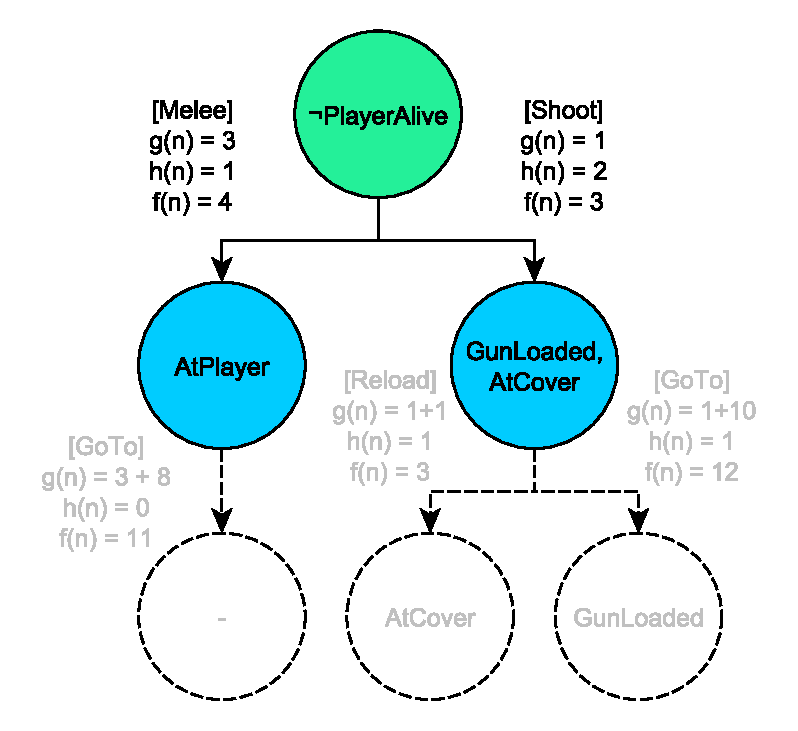
\includegraphics[width=0.5\textwidth]{GOAP/goap baum 1}
	\captionsetup{justification=justified, format=plain}
  \caption{GOAP A* Suche: Gr\"{u}ne Knoten sind Knoten, welche erweitert wurden. Blaue Knoten sind Knoten aus der offenen Liste.}
  \label{fig:goap1}
\end{figure}

Nun sucht der Planer alle m\"{o}glichen Aktionen die den Zielzustand erreichen ($\textit{ACTIONS}(s_z)$ $= {\textit{Shoot}, \textit{Melee}}$). Es werden nicht erf\"{u}llte und vorausgesetzte Zust\"{a}nde der gefundenen Aktionen, sowie die Kosten $g(n)$ und $f(n)$ in den Knoten hinterlegt. Beide werden in die offene Liste hinzugef\"{u}gt.

Zur weiteren Suche entscheidet sich der A* Algorithmus f\"{u}r den Knoten mit den geringsten Kosten aus der offenen Liste, welcher durch die Bewertungsfunktion $f(n) = g(n) + h(n)$ berechnet wurde. Die Kosten $g(n)$ werden durch die $\textit{ACTIONCOST}$-Funktion gelesen. Die Heuristik $h(n)$ stellt sich durch die Summe an noch nicht erf\"{u}llten Zust\"{a}nden. Im Beispiel expandiert A* den Knoten \textit{GunLoaded, AtCover} der durch die Aktion \textit{Shoot} generiert wurde. Der Zustand \textit{AtPlayer} bleibt weiterhin in der offenen Liste.

\begin{figure}[h]
  \centering
  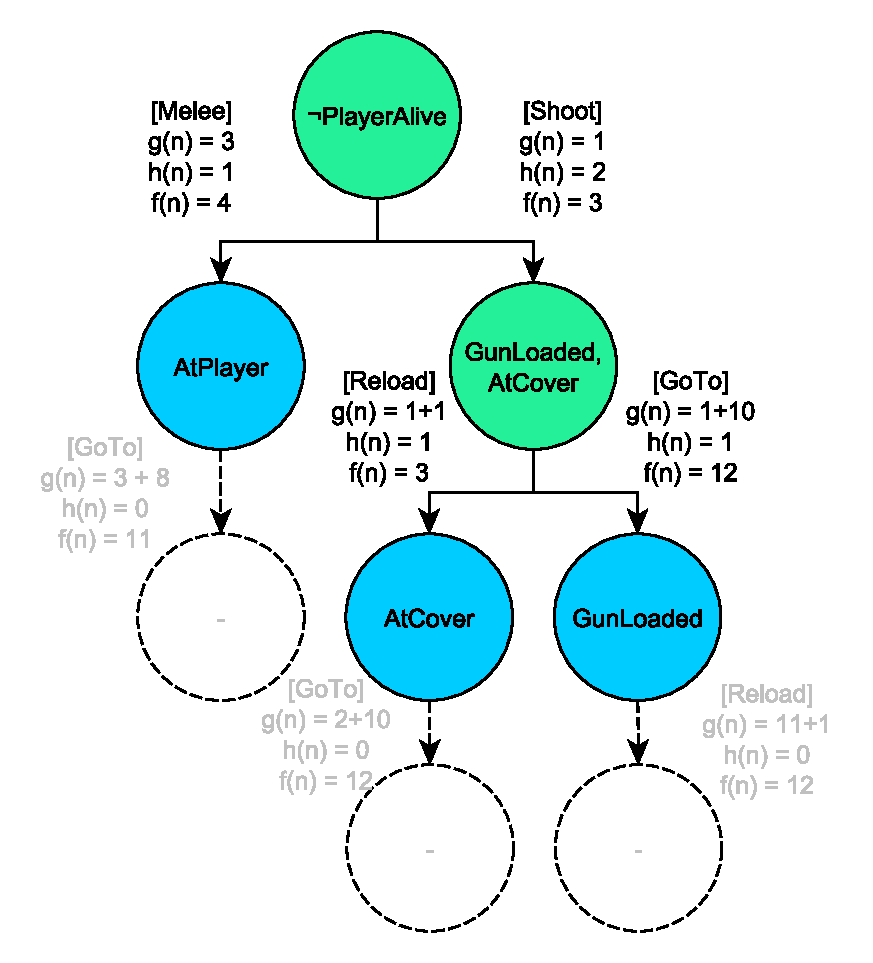
\includegraphics[width=0.6\textwidth]{GOAP/goap baum 2}
	\captionsetup{justification=justified, format=plain}
  \caption{GOAP A* Suche}
  \label{fig:goap2}
\end{figure}

F\"{u}r den expandierten Knoten \textit{GunLoaded, AtCover} werden nun Aktionen gesucht, die die Zust\"{a}nde des Knoten erf\"{u}llen. In dem Beispiel sind es \textit{Reload} und \textit{GoTo}. Auch die Knoten die durch die Aktionen entstehen, werden in die offene Liste hinzugef\"{u}gt. Erneut w\"{a}hlt A* den Knoten mit den geringsten Kosten $f(n)$ zur Expansion.
\clearpage

\begin{figure}[h]
  \centering
  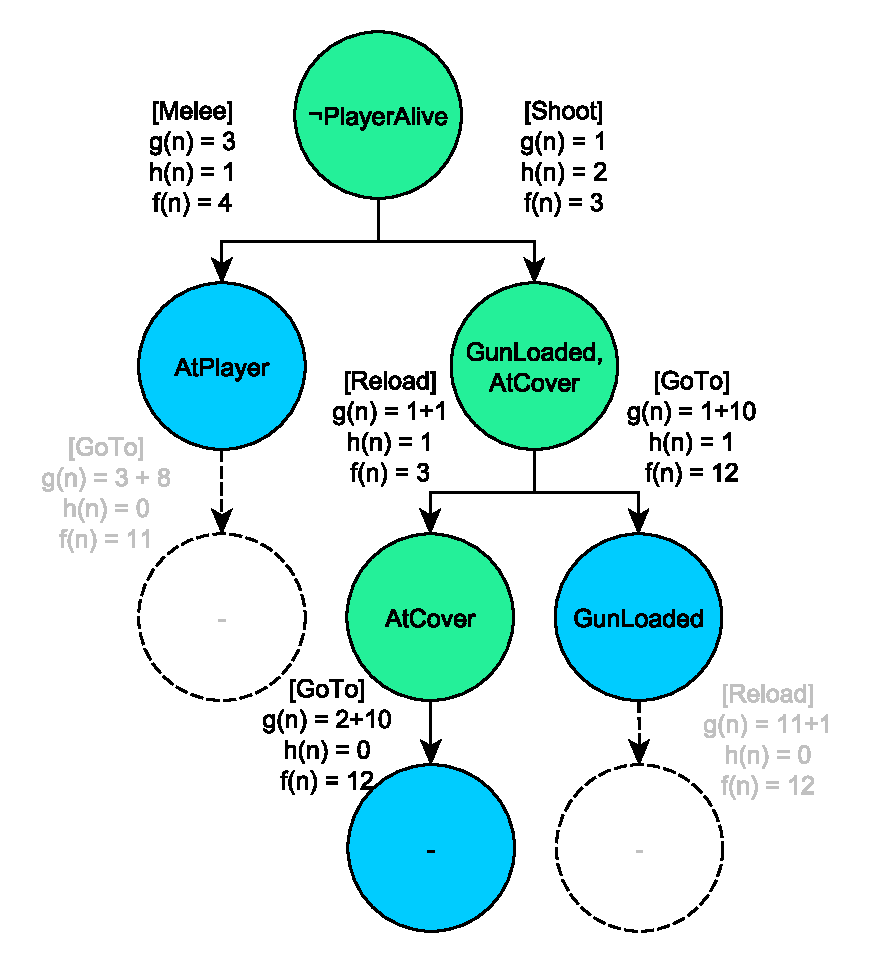
\includegraphics[width=0.6\textwidth]{GOAP/goap baum 3}
	\captionsetup{justification=justified, format=plain}
  \caption{GOAP A* Suche}
  \label{fig:goap3}
\end{figure}

Der Knoten der durch die Aktion \textit{Reload} entstand, hat dabei die geringsten $f(n)$ Kosten. Der nachfolgende Knoten, der durch die Aktion \textit{GoTo} erzeugt wird, hat zwar einen leeren Zustand und w\"{a}re somit abgeschlossen, befindet sich jedoch gemeinsam mit dem \textit{AtPlayer}-Knoten, der geringere Kosten hat, noch in der offenen Liste.

\begin{figure}[h]
  \centering
  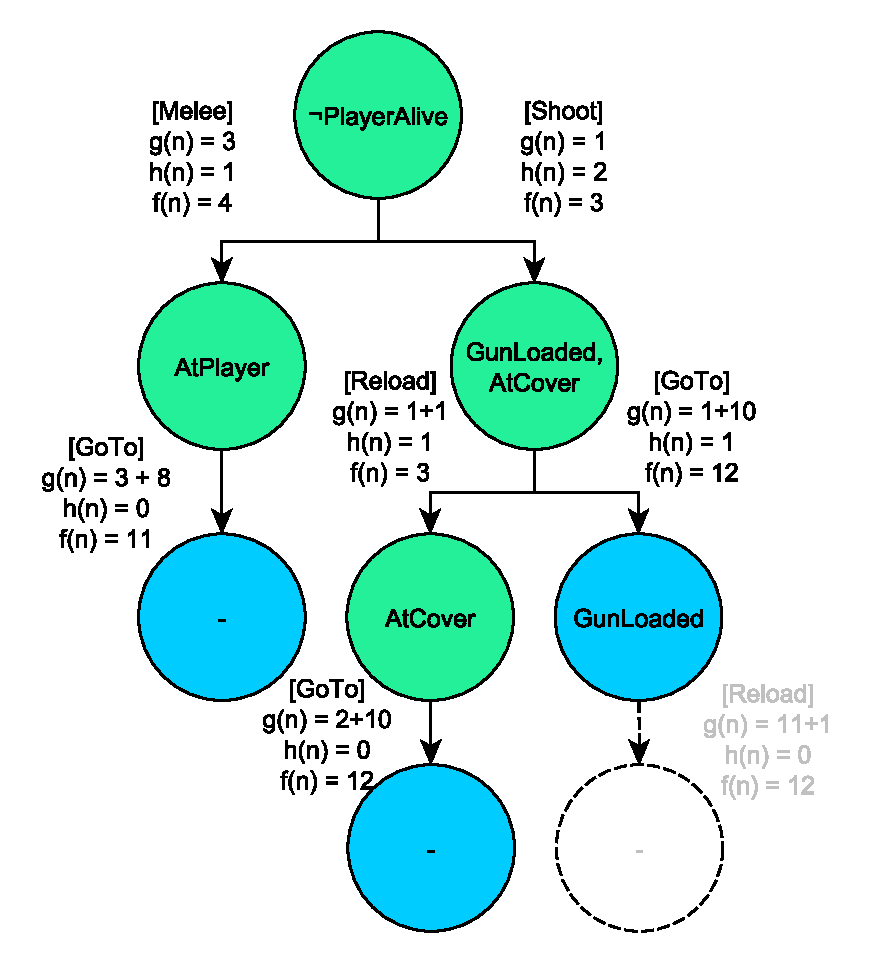
\includegraphics[width=0.6\textwidth]{GOAP/goap baum 4}
	\captionsetup{justification=justified, format=plain}
  \caption{GOAP A* Suche}
  \label{fig:goap4}
\end{figure}

Aus der offenen Liste wird der n\"{a}chste Knoten mit dem Zustand \textit{AtPlayer} gew\"{a}hlt, da dieser die niedrigsten Kosten von allen anderen offenen Knoten hat. Dieser wird durch die Aktion \textit{GoToPlayer} erf\"{u}llt und f\"{u}hrt zu einem Knoten mit leerem Zustand.

\begin{figure}[h]
  \centering
  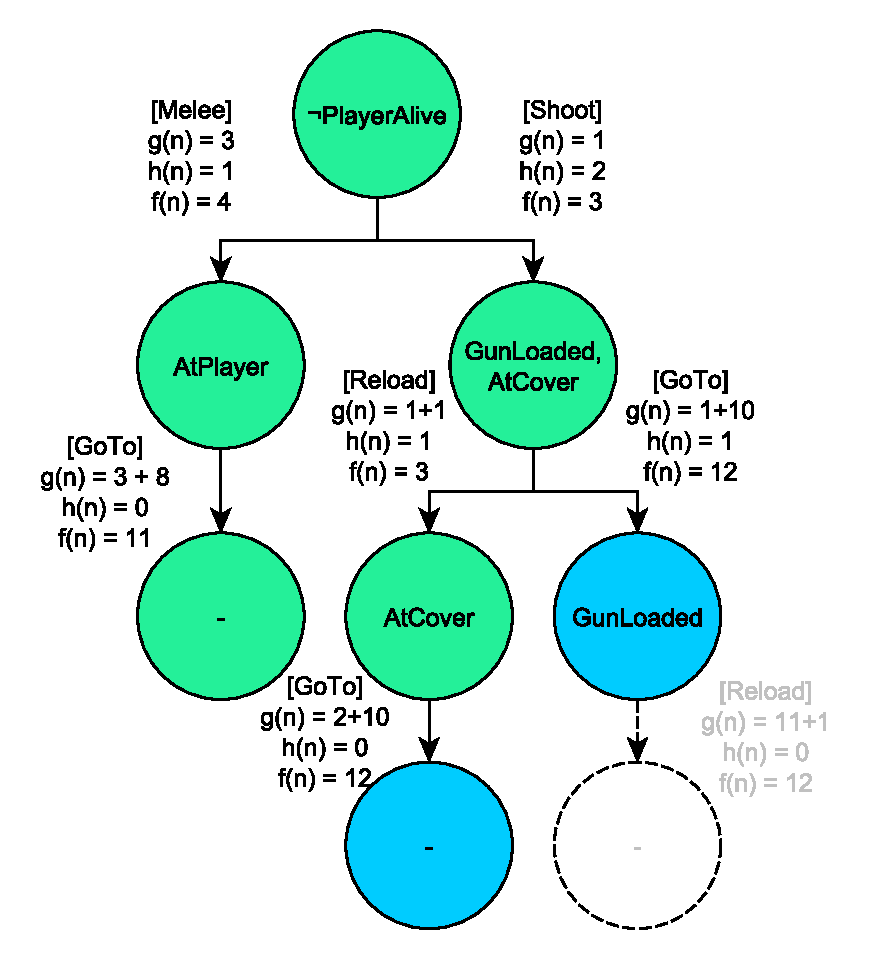
\includegraphics[width=0.6\textwidth]{GOAP/goap baum final}
	\captionsetup{justification=justified, format=plain}
  \caption{GOAP A* Suche}
  \label{fig:goap5}
\end{figure}

Letztlich wird der g\"{u}nstigste Knoten aus der offenen Liste genommen. Da dieser erf\"{u}llt ist, beziehungsweise keine weiteren Zust\"{a}nde besitzt, gibt der Planer nun die Goap-Aktionen, also die Kanten, die zu ihm gef\"{u}hrt habe in einer Aktions-Sequenz zur\"{u}ck. Im Beispiel w\"{a}re es die Aktions-Sequenz: [\textit{Melee, GoTo}]. Diese Aktions-Sequenz muss nun gespiegelt werden, da der A*-Suchalgorithmus vom Zielzustand angefangen hat. Somit w\"{a}re die richtige Aktions-Sequenz: [\textit{GoToPlayer, Melee}].